\documentclass{article}

\usepackage{amsmath,amsthm,amsfonts,amssymb,bm}
\addtolength{\textheight}{5.0cm}
\addtolength{\voffset}{-3.5cm}
\addtolength{\hoffset}{-2.5cm}
\addtolength{\textwidth}{4.0cm}

\allowdisplaybreaks

\usepackage{subeqnarray}
\usepackage{mathrsfs}
\usepackage[usenames,dvipsnames]{color}
\usepackage{url}
\usepackage{ulem}
\usepackage{indentfirst}
%\usepackage{textcomp}
%\usepackage{graphics}
\usepackage{graphicx}
\usepackage[hang,small,bf]{caption}
\setlength{\captionmargin}{50pt}

%includeonly{}


\graphicspath{{Figures/}{Figures/CPL/}{Figures/DE/}{Figures/P/}{Figures/DESync/}{Figures/DESync/DEs_Sync3/}}


%\usepackage{tikz}
%\usetikzlibrary{mindmap,trees}

\begin{document}
\title{Power Spctrum \& Its Evolution}
\author{MA Lei}
\maketitle


%%%%%%%%%%%%%%%%%%%%%%%%%%%%%%%%%%%%%%%%%%%%%%%%%%%%%%%%%
%%%%%%%%%%%%%%%%%%%%%%%%%%%%%%%%%%%%%%%%%%%%%%%%%%%%%%%
%%%%%%%%%%%%%%%%%%%%%%%%%%%%%%%%%%%%%%%%%%%%%%%%%%%%%%%%
%%%%%%%%%%%%%%%%%%%%%%%%%%%%%%%%%%%%%%%%%%%%%%%%%%%%%%%
%%%%%%%%%%%%%%%%%%%%%%%%%%%%%%%%%%%%%%%%%%%%%%%%%%%%%%%



Figure \ref{fig:DE_HubbleDistance2_Sync} shows several ratios of the Hubble distance.
 
 
Figure \ref{fig:GrowthFunction_Sync} and figure \ref{fig:GrowthFunction_Sync2} are the growth functions.

Figure \ref{fig:PowerSpectrum_Sync} is the power spectra.

Figure \ref{fig:DE_Qfac_Sync} shows the normalization factors, which are defined as 
\begin{equation}
Q^2=\frac{\text{Power spectra of DE model with EoS w}}{\text{Power spectra of LCDM model}}, \text{at some wavenumber $k$.}
\end{equation}


\newpage    %It is weird that this command solve the problem that the figure goes between the double line and the text.
\hrule\vspace{1pt}\hrule
\begin{center}
\mbox{{\bf XXXX}} \\
\vspace{0.5em}
\mbox{{XXXX}}
\end{center}
\hrule






\begin{figure}[!htbp]
\centering
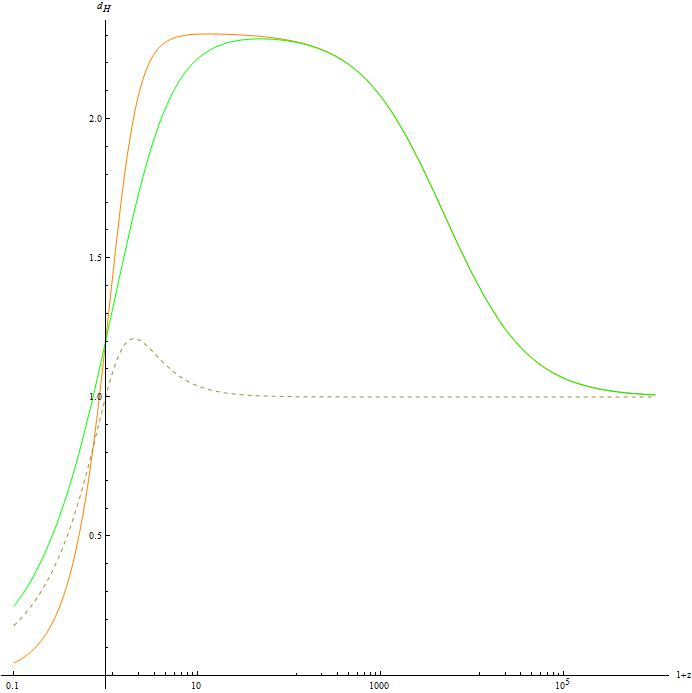
\includegraphics[width=500pt]{DEs_HubbleDistance_Sync.jpg}
\caption{Hubble distance with a legend}\label{fig:DE_HubbleDistance2_Sync}
\end{figure}





\begin{figure}[!htbp]
\centering
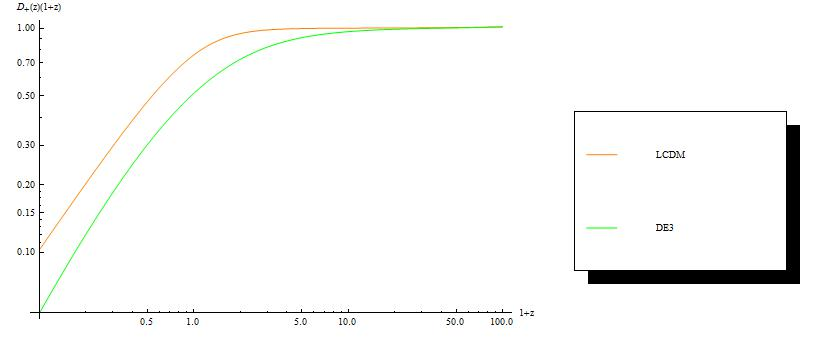
\includegraphics[width=400pt]{DEs_GrowtheFunction_Sync.jpg}
\caption{Growth function}\label{fig:GrowthFunction_Sync}
\end{figure}


\begin{figure}[!htbp]
\centering
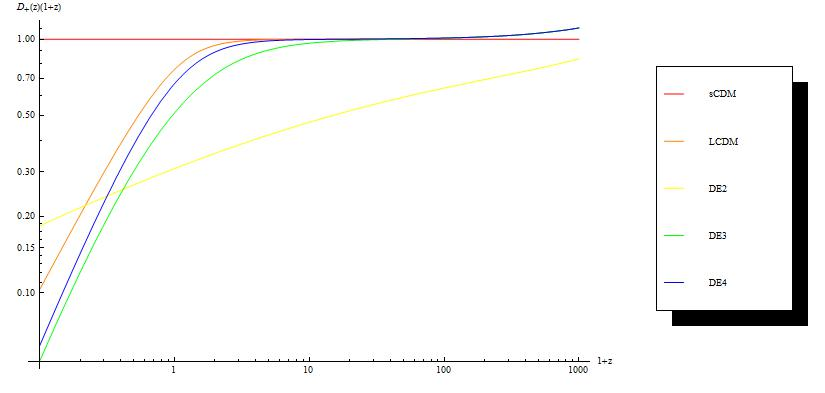
\includegraphics[width=400pt]{DEs_GrowtheFunction_Sync2.jpg}
\caption{Growth function}\label{fig:GrowthFunction_Sync2}
\end{figure}








\begin{figure}[!htbp]
\centering
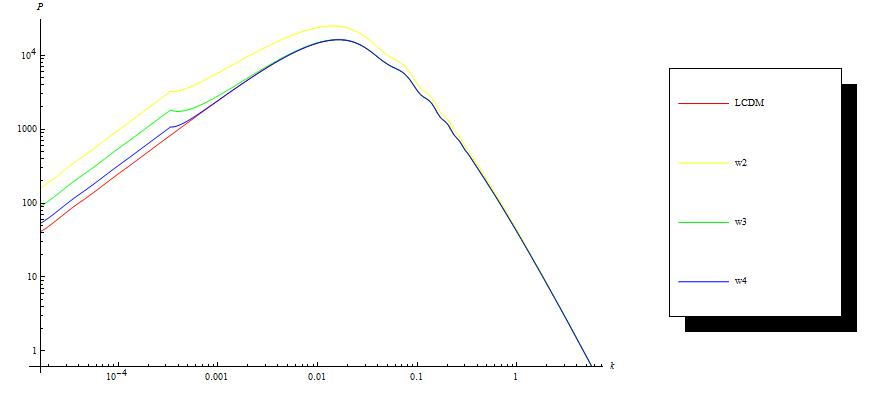
\includegraphics[width=400pt]{DEs_PowerSpectrum_Sync.jpg}
\caption{Power spectrum}\label{fig:PowerSpectrum_Sync}
\end{figure}



\begin{figure}[!htbp]
\centering
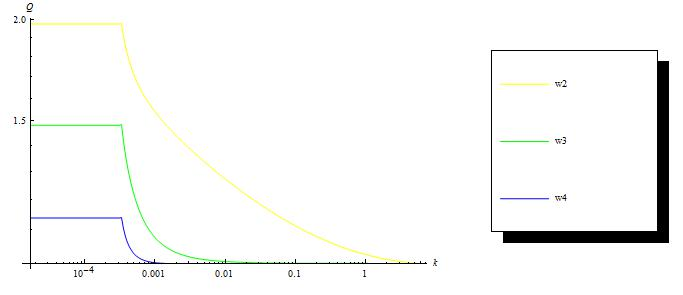
\includegraphics[width=400pt]{DEs_Q_Sync.jpg}
\caption{Q factors}\label{fig:DE_Qfac_Sync}
\end{figure}



















%%%%%%%%%%%%%%%%%%%%%%%%%%%%%%%%%%%%%%%%%%%%%%%%%%%%%%%%%
%%%%%%%%%%%%%%%%%%%%%%%%%%%%%%%%%%%%%%%%%%%%%%%%%%%%%%%
%%%%%%%%%%%%%%%%%%%%%%%%%%%%%%%%%%%%%%%%%%%%%%%%%%%%%%%%
%%%%%%%%%%%%%%%%%%%%%%%%%%%%%%%%%%%%%%%%%%%%%%%%%%%%%%%
%%%%%%%%%%%%%%%%%%%%%%%%%%%%%%%%%%%%%%%%%%%%%%%%%%%%%%%
\end{document}